\documentclass[tikz,border=6pt]{standalone}
\usepackage[T1]{fontenc}
\usepackage{lmodern}
\usepackage{amsmath,amssymb}
\usetikzlibrary{arrows.meta,angles,quotes,calc,positioning}
\definecolor{axis}{HTML}{40515F}
\definecolor{grid}{HTML}{DDE4E8}
\definecolor{blue}{HTML}{3568D4}
\definecolor{coral}{HTML}{EF626C}
\definecolor{teal}{HTML}{2A9D8F}
\definecolor{gold}{HTML}{D89432}
\definecolor{purple}{HTML}{7357C8}
\tikzset{
  axisline/.style={axis, line width=.85pt, -{Stealth[length=3mm]}},
  guide/.style={axis!45, line width=.75pt, dashed},
  vector/.style={line width=1.5pt, -{Stealth[length=3mm]}},
  dot/.style={circle, fill=white, draw, line width=1.15pt, inner sep=2.15pt},
  label/.style={font=\large},
  smalllabel/.style={font=\normalsize}
}
\begin{document}

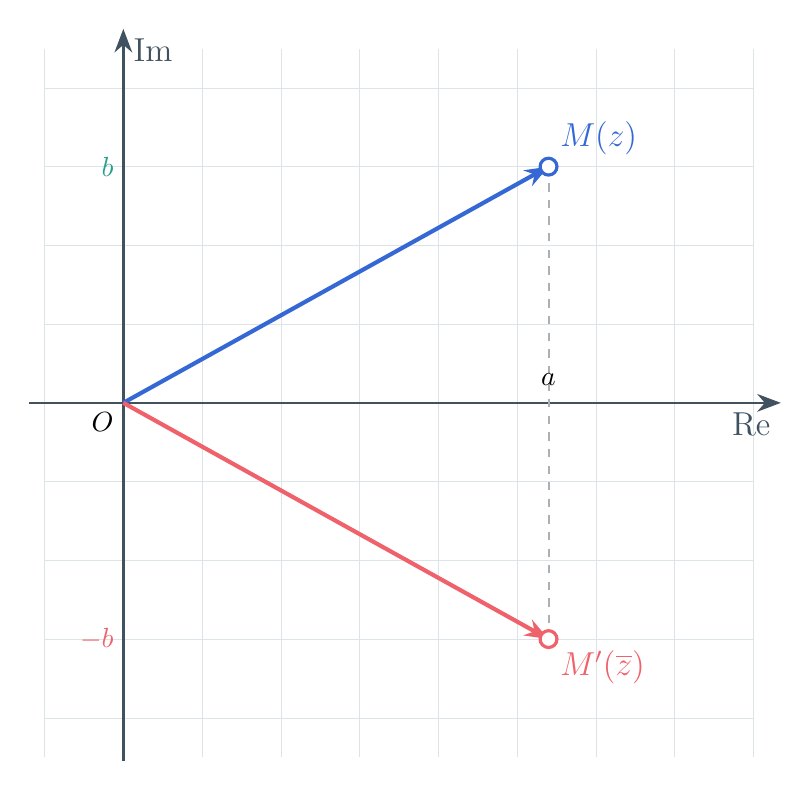
\begin{tikzpicture}[x=1cm,y=1cm]
  \draw[step=1cm,grid,very thin] (-1,-4.5) grid (8,4.5);
  \draw[axisline] (-1.2,0)--(8.35,0) node[below left,font=\large] {$\operatorname{Re}$};
  \draw[axisline] (0,-4.55)--(0,4.75) node[below right,font=\large] {$\operatorname{Im}$};
  \coordinate (O) at (0,0);
  \coordinate (M) at (5.4,3);
  \coordinate (Mb) at (5.4,-3);
  \draw[guide] (M)--(Mb);
  \draw[vector,blue] (O)--(M);
  \draw[vector,coral] (O)--(Mb);
  \node[dot,draw=blue] at (M) {};
  \node[dot,draw=coral] at (Mb) {};
  \node[label,blue,above right=1pt of M] {$M(z)$};
  \node[label,coral,below right=1pt of Mb] {$M'(\overline z)$};
  \node[smalllabel] at (5.4,.3) {$a$};
  \node[smalllabel,teal,left] at (0,3) {$b$};
  \node[smalllabel,coral,left] at (0,-3) {$-b$};
  \node[smalllabel,below left] at (O) {$O$};
\end{tikzpicture}
\end{document}
